\chapter{Weak Memory Models}
\label{ch:wmm}

%"Semantics and verification under weak memory models have been the subject of study at least since 2007." [PORTHOS]
The \textit{weak memory model} is a set of predicative constraints on possible executions of a concurrent program. The study of formalisation weak memory models for different architectures has been rapidly developed over last decade. 

Firstly, the research of WMM aimes to formalise the weak memory models and provide systematic, sound and complete formal approach of defining WMMs in order to be able to verify systems with respect to them.
A generic framework of program analysis with respect to weak memory models was presented in 2010~\cite{alglave2010shared}. Similar approach is used \texttt{PORTHOS} as it is described
% in Section~\cite{ch:wmm:event}. 
further in current Chapter.

Secondly, researchers work on extracting the WMMs of hardware architectures from existing implementations of from their specifications, that are written in natural language and thus suffer from ambiguities and incompletenesses. Over last decade the memory models have been extracted for most mainstream multiprocessor architectures, such as x86-TSO (\textit{Total Store Order}) model for x86 architecture formalised in 2009~\cite{owens2009better}, much more relaxed memory model for Power and ARM architectures~\cite{alglave2009semantics,sarkar2011understanding}, for Alpha~\cite{?} and Sparc~\cite{?} memory models were defined in the specification. Moreover, most modern high-level programming languages rely on relaxed memory model. Thus, the memory model for Java that is based on the \textit{happens-before} principle~\cite{lamport1978time} was introduced in J2SE 5.0 in 2004~\cite{manson2005java}; the C++11 standard~\cite{?} has introduced the set of hardware-independent synchronisation fences and atomic operations, whenever the C++17 memory model is based on the relation \textit{strongly happens-before}.
%batty2011mathematizing

Thirdly, important research direction targets the problem of verifying (or at least finding bugs in) existing software systems with respect to weak memory models. Perhaps, the most notable work in this field is the project for defining the Linux kernel memory model, which is being actively developing these days~\cite{kernel1}.
%Distributed databases <also need the wmm, see transaction consistency~\cite{bailis2013highly}>

%experiments with kernel?

\section{The event-based program representation}
\label{ch:wmm:event}

%"The semantics of a program is a set of executions" https://johnwickerson.github.io/papers/memalloy.pdf

The classical approach to model the concurrent programs is to use the \textit{global time}, a single order of interleavings of all actions happened in different threads. However these models are easy to understand, it may be hard to consider \textit{all} possible states, number of which is exponentially large. Another way to do this is to to use non-deterministic computation-centric models defined in~\cite{fri97}, one of which represents the program as the graph of \textit{memory events}. The idea in this class of models is based on the fact that the behaviour of a concurrent system is defined only by the interleavings of shared-memory operations, while being independant from the order of local computation events. These models may be further restricted by constraints of a weak memory model, adding \textit{relations} to the memory events.
%Perhaps, the most convenient way to model the non-deterministic properties of concurrent programs is to use the program representation based on \textit{memory events}.
%In order to model the non-deterministic properties of concurrent programs 

The event-based program model represents the directed graph (\textit{event-graph}), where vertices represent \textit{events}, and edges represent \textit{relations} over the events. An event is something, that, after being executed, changes the state of an abstract machine executing the concurrent program. 
An \textit{execution} (trace, run) of a given program is an ordered set of events.
%associated with the instructions of the program
%the path in the event-graph. 
An execution is considered to be \textit{valid} if the memory events follow a single global timeline, i.e., can be embedded in a single partial order allowed by the memory model restrictions~\cite{alglave2010shared}. An execution to be checked on validity is called the \textit{candidate execution}.

Below we describe some basic types of events and relations.

\subsection{Events}
\label{ch:wmm:model:events}

A \textit{memory event} $e_m \in \mathbb{E}$ represents the fact of access to the memory. Since memory is the crucial low-level resource shared by multiple processes, most relations are defined over memory events. 
The processes can access a shared memory location (denoted by~$l_i$, for \textit{location}), or a local one (denoted by~$r_i$, for \textit{register}). A memory event is specified by its direction with respect to the shared variable, its location~$\texttt{loc}(e_m)$, its processor label~$\texttt{proc}(e_m)$, and a unique event label~$\texttt{id}(e_m)$~\cite{alglave2010shared}. 
%\texttt{load} for read the value of a shared-memory location, or \texttt{store} for write, or neither of them if both locations are local
The set of memory events $\mathbb{M}$ is devided into write events $\mathbb{W}$ (that write values to shared-memory locations) and read events $\mathbb{R}$ (that read values stored in shared-memory locations).
We add a restriction that each memory event uses at most one shared location, so that the write event $e_m = write(l_1, l_2)$ that writes value from shared location $l_2$ to the shared location $l_1$ is represented as two consequent events $e_m'~=~\texttt{load}(r_1 \leftarrow l_2); \ e_m''~=~\texttt{store}(l_1 \leftarrow r_1)$.

A \textit{computation event} $e_c \in \mathbb{C} \subseteq \mathbb{E}$, represents a low-level assembly computation operation performed solely on local-memory arguments. An example of computation event may be the event $e_c = r_3 \leftarrow add(r_1, r_2)$ that writes the sum of values stored in registers $r_1$ and $r_2$ to the register $r_3$. The \textit{control-flow} instructions (conditional and unconditional jumps) are encoded to the model directly, without additional events, as the $po$-relation (for \textit{program order}; see Chapter~\ref{ch:wmm:model:relations} for detailed definition of relations).

The third class of events is \textit{barrier events}, events caused by the synchronisation instructions (called \textit{fences}). Barrier events do not perform any computation or memory value transfer, instead, they add new relations to the model that restrict the set of allowed behaviours. Technically, a fence may either serve as a synchronisation barrier, or flush local memory caches, etc.


\subsection{Relations}
\label{ch:wmm:model:relations}

The basic relation in the event-based program model is the \texttt{po}-relation $\subset~\mathbb{E}~\times~\mathbb{E}$ (\textit{program-order}), which represents the total order of memory events \textit{within single process}, which never relates events from different processes. Thus, if a program specifies the memory instruction $i_2$ to follow immideately the memory instruction $i_2$, then there exist an edge $e_1 \xrightarrow{\texttt{po}} e_2$ in the event-graph where event $e_1$ is caused by the instruction $i_1$ and $e_2$ is caused by the instruction $i_2$. This relation encodes the control-flow of the program into the event-graph.
%Some new relations may be acquired : dp, po-loc

The data-flow of a program is encoded by the \textit{communication relations}: the \texttt{rf}-relation $\subset~\mathbb{W}~\times~\mathbb{R}$ (\textit{read-from} relation) that maps a write to a read reading its value, the \texttt{co}-relation $\subset~\mathbb{W}~\times~\mathbb{W}$ (\textit{coherence order}, sometimes called \texttt{ws}-relation for \textit{write serialisation}) defines the total order on writes to the same location across all processes, and the \texttt{fr}-relation $\subset~\mathbb{R}~\times~\mathbb{W}$ (\textit{from-read order}) that maps a read to possible writes preceding the current write event.
%TODO: perephrase last sentence! alglave thesis, p. 36

Figure~\ref{simple_wmm_x86_pic} illustrates the candidate execution for the Example~\ref{simple_wmm_x86}, that reaches the state \texttt{(0:EAX=0~/\textbackslash~1:EAX=0)} within x86-TSO memory model (the picture is generated by the \texttt{herd7} tool, version 7.47). 
%The event $b$:\texttt{(Ry=0)} reads value \texttt{0} at the shared location \texttt{y} from the initial write event $e$\texttt{(Wy=0)} (the red edge of \texttt{rf}-relation), consequently, 
%the event $d$:\texttt{(Rx=0)} reads value \texttt{0} at the shared location \texttt{x} from the initial write event $f$\texttt{(Wx=0)} (the red edge of \texttt{rf}-relation). 

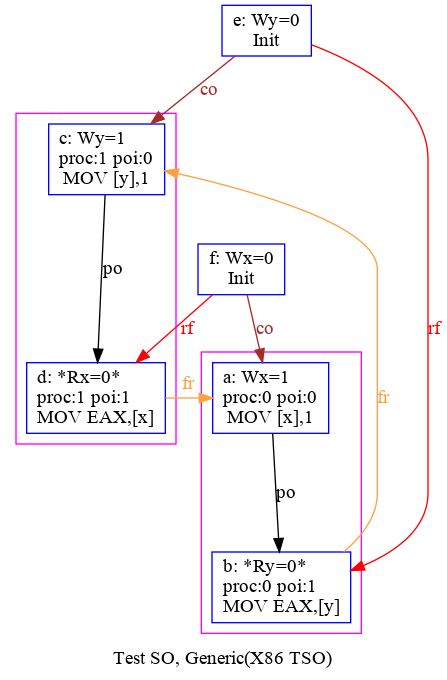
\includegraphics[width=0.4\textwidth]{img/my/simple_wmm_x86.png}
\label{simple_wmm_x86_pic}
% TODO: re-generate with new name, not 'SO'

\subsection{Executions}
\label{ch:wmm:model:executions}

The semantics of a concurrent program is represented by the set of allowed executions.
An execution is uniquely defined by the set $\mathbb{X}$ of events have been executed in each thread (the \textit{control-flow} of a program), and the relations $\mathtt{rf}$ and $\mathtt{co}$ (\textit{data-flow} of a program)~\cite{alglave2010shared}. As it was shown in~\cite{wickerson2017automatically}, it is enough for memory models to constrain the executions independently instead of constraining the program as a whole.

\section{The CAT language}

The Porthos tool uses the language \texttt{CAT}~\cite{alglave2016syntax} for defining weak memory models.

the event representation

\section{Some known WMM}

\subsection{x86-TSO}
\label{ch:wmm:x86}
// exmaple with reordering
// ex. with 
// Rev-29 Example 7-6. Stores Are Transitively Visible. %see http://www.cl.cam.ac.uk/~pes20/weakmemory/x86tso-paper.pdf

There is a barrier instruction \texttt{mfence} that may be used for flushing the buffers into the main memory.

briefly known hw memory models: X86-TSO, Alpha, POWER, -- ref to Jade;
language memory models: Java, C++;
library-level kernel memory model, ref to github with tests

Relationship between different models \url{http://wiki.expertiza.ncsu.edu/index.php/CSC/ECE_506_Spring_2013/10c_ks}
